% CHAPTER
\chapter{Composite polynomial approximation to \texorpdfstring{$\sgn (x)$}{sgn(x)}}\label{sgnchapter}

\section{Zolotarev functions}

To motivate the work of this chapter, we first discuss a notable result in rational approximation theory, concerning the rational best approximations to $\sgn(x)$ on 
\[X(\delta)=[-1,-\delta]\cup [\delta,1],\] 
for some $\delta \in (0,1)$. Such approximations are referred to as the \textit{Zolotarev functions}; in particular, we write $Z_{2r+1}(x;\delta)$ for type $(2r+1,2r)$ approximations. The explicit form of $Z_{2r+1}(\cdot;\delta)$ was found by Zolotarev \cite{Zolo} in terms of Jacobi elliptic functions
\[\text{sn}(u;\delta)=\sin \phi, \qquad \text{cn}(u;\delta)=\cos \phi;\]
here $\phi$ denotes the Jacobi amplitude, obtained from the inversion of the \textit{incomplete elliptic integral of the first kind} (see e.g. \cite[Chapter 5]{akhiezer})
\[u=F(\phi;\delta):=\int_0^\phi \dfrac{d\theta}{\sqrt{1-\delta^2\sin^2 \theta}}.\]
The Zolotarev functions are then given by
\begin{align}
    Z_{2r+1}(x;\delta)=Mx\prod_{i=1}^r \dfrac{x^2+c_{2i}}{x^2+c_{2i-1}}, \label{zolotarevfn}
\end{align}

\begin{figure}[t!]
\centering
   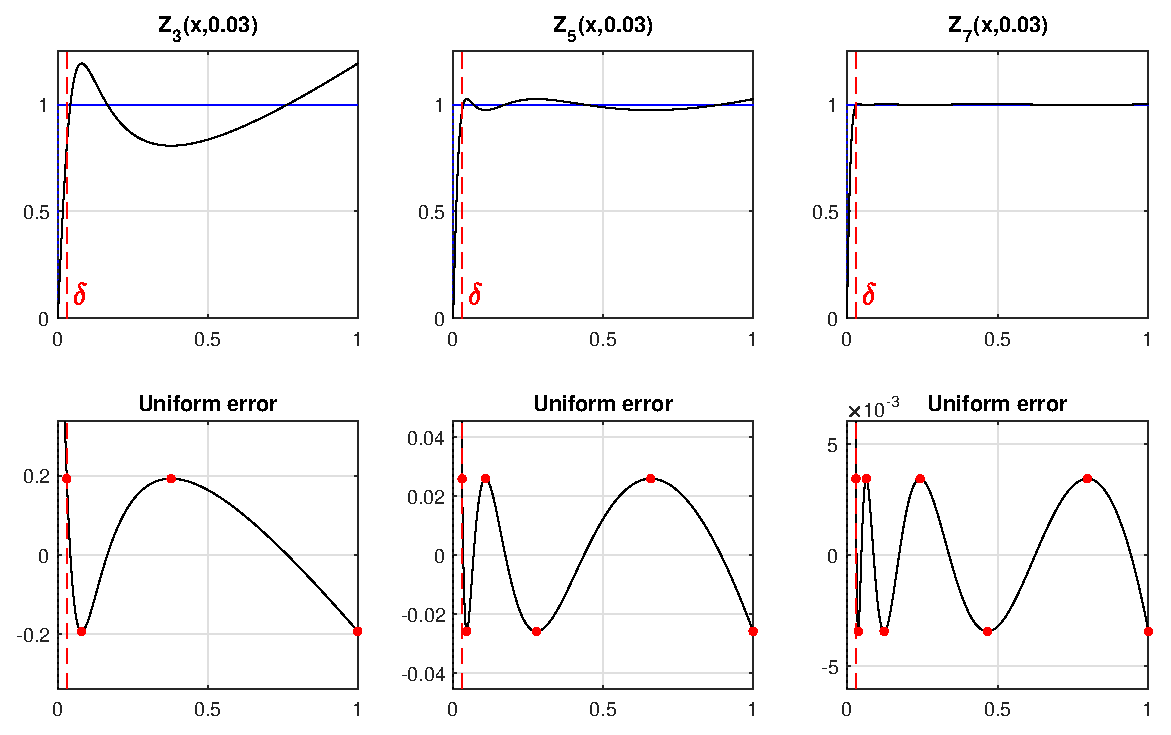
\includegraphics[width=\textwidth,height=\textheight,keepaspectratio]{figures/chapter_3/ZOLOTAREV.eps}
   \caption{Zolotarev functions $Z_{2r+1}(x;\delta)$ for $\delta=0.03$, constructed using \texttt{ellipke} and \texttt{ellipj}. The corresponding uniform error $\sgn(x)-Z_{2r+1}(x;\delta)$ is sketched below each plot, which equioscillates between $4r+4$ extrema in each case.}
   \label{fig:ZOLOT}
\end{figure}

where for $i=1,\dots,2r$ the constants $c_i$ are defined by
\[c_i=\delta^2 \dfrac{\text{sn}^2\left(\frac{iK'}{2r+1};\delta'\right)}{\text{cn}^2\left(\frac{iK'}{2r+1};\delta'\right)},\]
with $\delta'=\sqrt{1-\delta^2}$ and $K'=F(\pi/2;\delta')$ respectively denoting the \textit{complementary modulus} and \textit{complete elliptic integral of the first kind} for $\delta'$. Here, $M>0$ is a scalar determined by the equioscillation property of the best approximation, which ensures that $1-Z_{2r+1}(\delta;\delta)=-(1-Z_{2r+1}(1;\delta))$. Hence
\[M=2\left(\prod_{i=1}^r\dfrac{1+c_{2i}}{1+c_{2i-1}}+\delta \prod_{i=1}^r\dfrac{\delta^2+c_{2i}}{\delta^2 +c_{2i-1}}\right)^{-1}.\]

Nakatsukasa and Freund showed that normalised Zolotarev functions $\hat{Z}_{2r+1}(\cdot;\delta)$, which take the form \eqref{zolotarevfn} multiplied by $1/Z_{2r+1}(1;\delta)$, satisfy a recursive optimality property. Explicitly, we can write
\[\hat{Z}_{2r'+1}(\hat{Z}_{2r+1}(x;\delta_1);\delta_2) = \hat{Z}_{(2r+1)(2r'+1)}(x;\delta_1),\]
where $\delta_2$ is such that $X(\delta_2)=\hat{Z}_{2r+1}(X(\delta_1);\delta_1)$ \cite[Theorem 3]{YujiZolotFreund}. The proof involves counting equioscillation points and invoking the minimax equioscillation property. We use this as motivation for constructing a composite polynomial approximation consisting of the composition of low-order best approximations to the sign function.

\section{Greedy approximation to \texorpdfstring{$\sgn(x)$}{sgn x} in \texorpdfstring{$\Pee_{(k,3)}^{\text{comp}}$}{P k,3 comp}}

In this section, we construct a pure composite polynomial approximation to $\sgn(x)$ on $X(\delta)$ using a greedy iterative process, namely an approximation of the form
\[f_{k+1}(x) = g_{k+1}(f_{k}(x)), \qquad k=1,2,\dots,\]
where each $g_{k+1} \in \Pee_3$ is the best approximation to $\sgn(x)$ on its domain $f_{k}(X(\delta))$. We start by finding the best polynomial approximant $p \in \Pee_3$ to $\sgn(x)$ on $X(\delta)$, which is an odd function by Lemma \ref{symm}, hence has the form
\[p(x)=x(A+Bx^2),\]
for some constants $A,B$ to be determined. For simplicity, we normalise $p$ such that $\norm{p}_{\infty,X(\delta)}=1$, and as such approximate a scaled version of the sign function $C\sgn(x)$, for some constant $C \in (0,1)$ determined by the normalisation of $p$. By Corollary \ref{disjoint}, we know that $C\sgn -p$ equioscillates between at least 6 extrema: to obtain equioscillation, we can impose
\begin{align}
    p(\delta)=p(1)=2C-1, \label{valueofC}
\end{align}
so that the maximum error $1-C$ is obtained at the points  $\pm 1, \pm \delta$, $\pm \xi$, where $\xi \in (\delta,1)$ is the extremal point such that $p(\xi)=1$. This gives us three conditions:

\begin{itemize}
    \item\makebox[2cm]{$p(\delta)=p(1)$\hfill} $\quad\Longrightarrow \quad (1-\delta)A+(1-\delta^3)B=0$;
    \item\makebox[2cm]{$p'(\xi)=0$\hfill} $\quad\Longrightarrow \quad A+3\xi^2B=0$;
    \item\makebox[2cm]{$p(\xi)=1$\hfill} $\quad\Longrightarrow \quad \xi A + \xi^3 B-1=0$.
\end{itemize}

Solving these equations, we find that the best approximation is
\begin{align}
     p(x)=\dfrac{x}{2\xi}\left(3-\dfrac{x^2}{\xi^2}\right), \qquad \xi=\sqrt{\dfrac{1+\delta+\delta^2}{3}},\label{xis}
\end{align}

\begin{figure}[t!]
\centering
   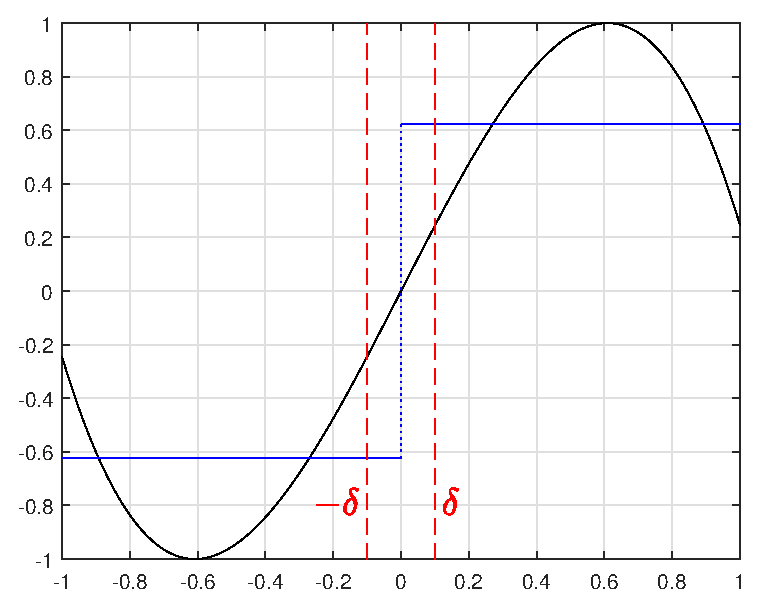
\includegraphics[width=0.6\textwidth,height=0.6\textheight,keepaspectratio]{figures/chapter_3/COMPSIGNsingle.eps}
   \caption{Best $\Pee_3$-approximation (black) to $C\sgn(x)$ (blue) on $X(\delta)$, where $\delta=0.1$.}
   \label{fig:compsign}
\end{figure}

By the symmetry of our construction, and using that $C=(1+p(\delta))/2$ by \eqref{valueofC}, we can obtain the maximum error $E$ in the approximation
\[E=1-C=\dfrac{1-p(\delta)}{2}.\]
Figure \ref{fig:compsign} sketches the approximation for $\delta=0.1$, for which the normalisation of $p$ gives $C\approx 0.6222$ and $E\approx 0.3778$.

\bigskip{}

\begin{rmk}
By symmetry, the range of $p$ is $X(p(\delta))$. In particular, the containment $X(p(\delta)) \subset X(\delta)$ is strict, thanks to the following lemma.
\end{rmk}

\begin{lemma}\label{tekky}
Given $\delta \in (0,1)$ and $p \in \Pee_3$ defined by \eqref{xis}, we have $p(\delta)>\delta$.
\end{lemma}

\begin{sproof}
There holds
\begin{align*}
    \dfrac{p(\delta)}{\delta} =\dfrac{1}{2\xi}\left(3-\dfrac{\delta^2}{\xi^2}\right)= \dfrac{3\sqrt{3}}{2}\left(\dfrac{1+\delta}{(1+\delta+\delta^2)^{3/2}}\right),
\end{align*}
so it remains to show that
\[\dfrac{3\sqrt{3}}{2}>\dfrac{(1+\delta+\delta^2)^{3/2}}{1+\delta}=:h(\delta).\]
But $h$ is strictly increasing, therefore $h(\delta)<h(1)=3\sqrt{3}/2$.
\end{sproof}

Fixing $p$ as in \eqref{xis}, we can similarly find the polynomial 
\[q \in \{f \in \Pee_3 : \norm{f}_{\infty,p(X(\delta))}=1\}\]
such that $q(p(x))$ is an optimal approximation for $D\sgn(x)$, for some scale factor $D$ determined by the normalisation of $q$. To see this, note that by the above remark, the domain of $q$ is $p(X(\delta))=X(p(\delta))$. Hence $q$ is obtained in the same manner as $p$, except with $\delta$ replaced by $p(\delta)$. Repeating this process, we obtain a sequence
\[f_{k+1}(x)=g_{k+1}(f_{k}(x)), \qquad k=0,1,2,\dots,\]
where $f_0(x)=x$ and
\begin{align}
    g_{k+1}(x) =\dfrac{x}{2\xi_{k+1}}\left(3-\dfrac{x^2}{\xi_{k+1}^2}\right), \qquad \xi_{k+1}=\sqrt{\dfrac{1+f_{k}(\delta)+f_{k}(\delta)^2}{3}}. \label{compconsts}
\end{align}

\begin{figure}[t!]
\centering
   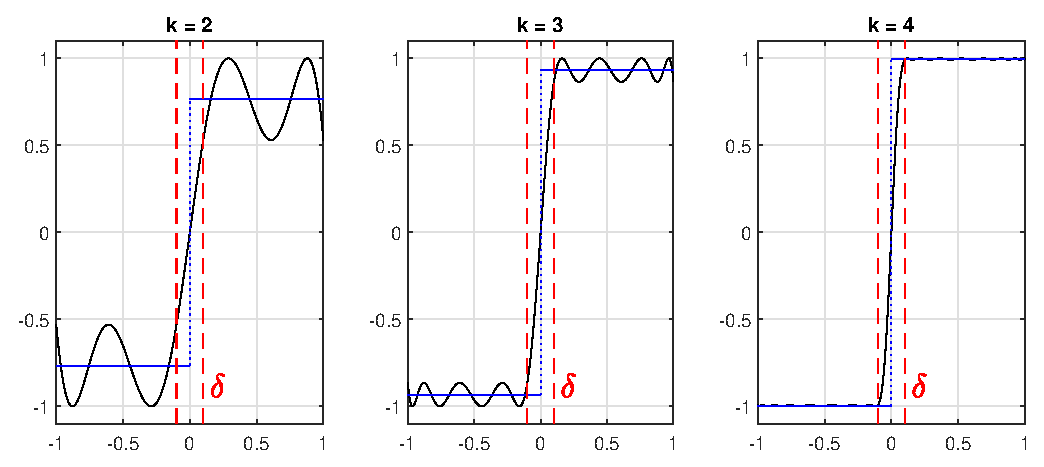
\includegraphics[width=\textwidth,height=\textheight,keepaspectratio]{figures/chapter_3/COMPSIGNthree.eps}
   \caption{Scaled Newton-Schulz iterates $f_k(x)$ (blue) with $C_k\sgn(x)$ (black) on $X(\delta)$, where $\delta=0.1$. The iterate for $k=1$ is shown in Figure \ref{fig:compsign}.}
   \label{fig:compsign2}
\end{figure}

By induction, it follows that $f_k \in \Pee_{(k,3)}^{\text{comp}}$, and is an approximation for $C_k \sgn(x)$ with maximum uniform error $E_k$, where 
\begin{align}
    C_k = \dfrac{1+f_k(\delta)}{2}, \qquad E_k = \dfrac{1-f_k(\delta)}{2}. \label{Ceekay}
\end{align}

\begin{rmk}
We note that $g_k(x) = g(x/\xi_k)$, where $g$ is the iteration function for the unscaled Newton-Schulz  approximation to the sign function \eqref{scalarNSsign}. Hence the iteration \eqref{compconsts} is equivalent to a scaled version of the of \eqref{scalarNSsign}, with $x$ replaced by $x/\xi_k$ at the $k^{\text{th}}$ iteration. As such, we will refer to \eqref{compconsts} as \textit{scaled Newton-Schulz} iterates to the sign function.
\end{rmk}

\section{Equioscillation behaviour}\label{equiSNS}

Since the scaled Newton-Schulz iterate $f_k$ has degree $3^k$, it follows by Corollary \ref{disjoint} that it is the best $\Pee_{3^k}$-approximation if $f_k-C_kf$ equioscillates between at least $3^k+3$ extrema on $X(\delta)$. By symmetry, this is the case when $f_k-C_k$ equioscillates between $(3^k+3)/2$ extrema on $[\delta,1]$. In the following technical lemma, we show that $f_k-C_k$ falls short of this number of equioscillation points.

\begin{figure}[t!]
\centering
   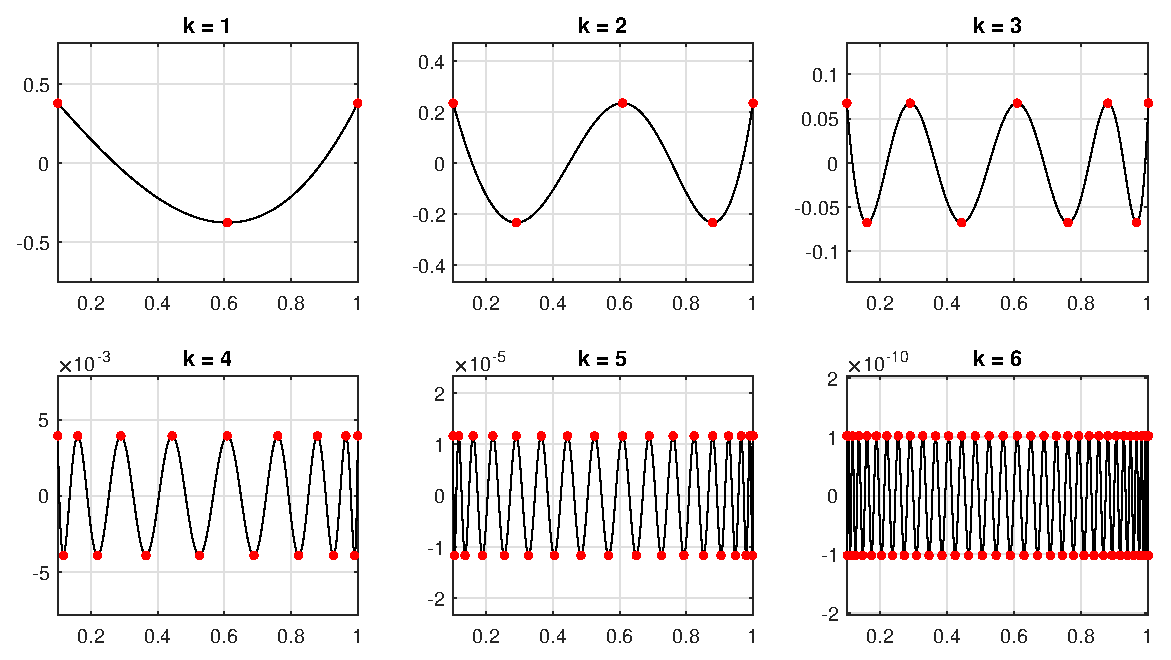
\includegraphics[width=\textwidth,height=\textheight,keepaspectratio]{figures/chapter_3/COMPSIGNMANYITERATES2.eps}
   \caption{Error $E_k(x)=C_k\sgn(x)-f_k(x)$ on $[\delta,1]$, where $\delta=0.1$. The error curve equioscillates between $2^{k}+1$ extrema in each case, as shown in Lemma \ref{equio}.}
   \label{fig:compsignmanyiterates}
\end{figure}

\begin{lemma}\label{equio}
Let $\delta \in (0,1)$ and $f_k \in \Pee_{(k,3)}^{\emph{comp}}$ be defined by \eqref{compconsts}. Then the error curve $f_k-C_k\emph{\sgn}$ equioscillates between $2^{k+1}+2$ extrema on $X(\delta)$, or equivalently, $f_k-C_k$ equioscillates between $2^{k}+1$ extrema on $[\delta,1]$.
\end{lemma}

\begin{proof}
By induction. The case for $k=1$ is clear, as we constructed $f_1$ to have 6 equioscillation points on $X(\delta)$. 

\bigskip{}

Now assume that $f_k-C_k \sgn$ equioscillates between $2^{k+1}+2$ extrema on $X(\delta)$, or equivalently between $2^k+1$ points $\{x_j\}_{j=1}^{2^k+1}$ on $[\delta,1]$. Then there are $2^k$ intervals $I_j=[x_j,x_{j+1}]$, $j=1,\dots,2^k$ such that $f_k(I_j)=[f_k(\delta),1]$.

\bigskip{}

Consider $g_{k+1}(x)$ on $[f_k(\delta),1]$. By construction, $g_{k+1}$ equioscillates between three points on this interval, namely $f_k(\delta)$, $\xi_{k+1}$ and $1$. Hence $g_{k+1}(f_k(x))$ equioscillates between 3 points on each $I_j$. Since we have $2^k$ such intervals, and $2^k-1$ points $\{x_j\}_{j=2}^{2^k}$ where equioscillation points overlap, the total number of equioscillation points of $g_{k+1}(f_k(x))$ on $[\delta,1]$ is
\[3(2^k) - (2^k-1)=2^{k+1}+1,\]
hence $2^{k+2}+2$ points on $X(\delta)$ by symmetry. But $g_{k+1}(f_k(x))=f_{k+1}(x)$, so this completes the inductive step of the theorem.
\end{proof}

\section{Convergence analysis of the scaled Newton-Schulz iterates}

We know from Section \ref{equiSNS} that the recursive optimality property of the Zolotarev functions \eqref{zolotarevfn} does not hold in the polynomial setting: composing normalised best cubic approximations to the sign function on $X(\delta)$ does not result in best approximations of higher order. However, we shall compare the convergence of the scaled Newton-Schulz iterates to the unscaled iterates and the minimax. In what follows, it will be useful to write $\delta_k:=f_k(\delta)$, so that \eqref{compconsts} reads
\begin{align}
    f_{k+1}(x) =\dfrac{f_k(x)}{2\xi_{k+1}}\left(3-\dfrac{f_k(x)^2}{\xi_{k+1}^2}\right), \qquad \xi_{k+1}=\sqrt{\dfrac{1+\delta_k+\delta_k^2}{3}}. \label{deltak}
\end{align}

\begin{figure}[t!]
\centering
   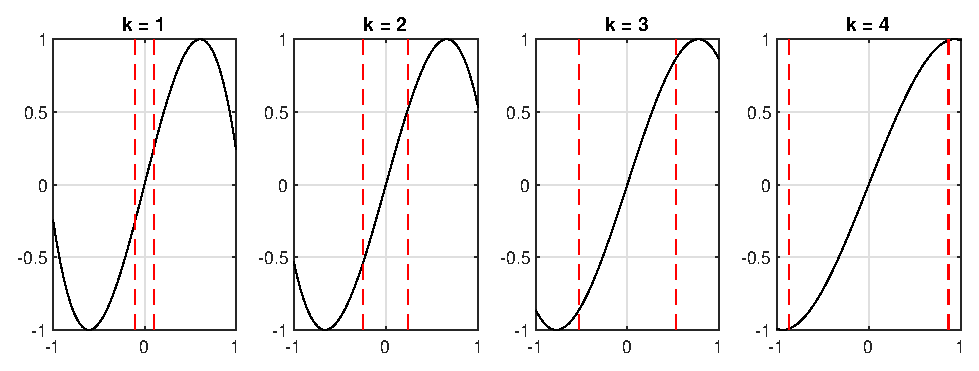
\includegraphics[width=\textwidth,height=\textheight,keepaspectratio]{figures/chapter_3/COMPSIGNiterationfunctions.eps}
   \caption{Iteration functions $g_k$ for the scaled Newton-Schulz iterates \eqref{deltak}. In each plot, the dotted red lines show the values of $\pm \delta_{k-1}$, starting with $\delta_0=\delta=0.1$.}
   \label{fig:compsigniterationfunctions}
\end{figure}

In particular, $\delta_k$ represents the value of $\delta$ used at the $(k+1)^{\text{st}}$ iteration to find the best cubic approximation to $C_{k+1} \sgn(x)$ on $X(\delta_k)$, as demonstrated in Figure \ref{fig:compsigniterationfunctions}. As a starting point, we have the formula
\[\ep_k:=\dfrac{E_k}{C_k}=\dfrac{1-\delta_k}{1+\delta_k},\]
which is the maximum uniform error $C_k^{-1}f_k-\sgn$. A comparison in the error of the scaled/unscaled Newton-Schulz iterates and the minimax approximation with respect to the degrees of freedom yields a striking result. Recall that the $k^{\text{th}}$ Newton-Schulz iterate (scaled or unscaled) has degree $3^k$, yet only $2k$ degrees of freedom\footnote{Each iteration function $g_k$ is an odd cubic polynomial, needing only two coefficients in terms of $\xi_k$ to be defined.}. However, the best approximation of degree $3^k$ requires $(3^k+1)/2$ degrees of freedom---half of a plain polynomial of degree $3^k$, since the best approximation is also an odd function). Therefore, the $k^\text{th}$ scaled or unscaled Newton-Schulz iterate has the same number of degrees of freedom as the minimax approximation of degree $4k-1$. 

\bigskip{}

\begin{figure}[t!]
\centering
   \includegraphics[width=0.7\textwidth,height=0.7\textheight,keepaspectratio]{figures/chapter_3/COMPSIGNvsBEST_DOFpoint1.eps}
   \caption{Comparison in the error of the Newton-Schulz, scaled Newton-Schulz and best approximants to $\sgn(x)$ on $X(\delta)$, where $\delta=0.1$, with respect to the degrees of freedom. The minimax is approximated using \texttt{polyvalA} and \texttt{polyfitA\_Lawson}\protect\footnotemark.}
   \label{fig:compsignvsbestDOF}
\end{figure}

Figure \ref{fig:compsignvsbestDOF} shows that the composite polynomial approximations are superior to the minimax with respect to degrees of freedom. Compared to \cite[Theorem 1]{Erem}, which shows that the minimax $p^*_m \in \Pee_{2m+1}$ to $\sgn(x)$ on $X(\delta)$ satisfies
\begin{align}
    \norm{p^*_m - \sgn}_{\infty,X(\delta)} \sim \dfrac{1-\delta}{\sqrt{\pi\delta}} m^{-1/2} \left(\dfrac{1-\delta}{1+\delta}\right)^m \label{eremboi}
\end{align}
as $m\to\infty$, we gain insight into why convergence of the minimax is much slower: despite being exponentially convergent, the term $\frac{1-\delta}{1+\delta}$ is very close to 1 for small values of $\delta$. A further observation from Figure \ref{fig:compsignvsbestDOF} is that, whereas the standard Newton-Schulz iterates perform worse than the minimax in the initial convergence phase, the scaled Newton-Schulz iterates are quick to outperform the minimax.

\bigskip{}

\footnotetext{Introduced by Brubeck, Nakatsukasa and Trefethen, these functions are adaptations of the standard \texttt{polyval} and \texttt{polyfit} methods---which fit polynomials to data using Vandermonde matrices---made stable by means of Arnoldi orthogonalisation. For details, see \cite{vandermonde}.}

\begin{figure}[t!]
\centering
   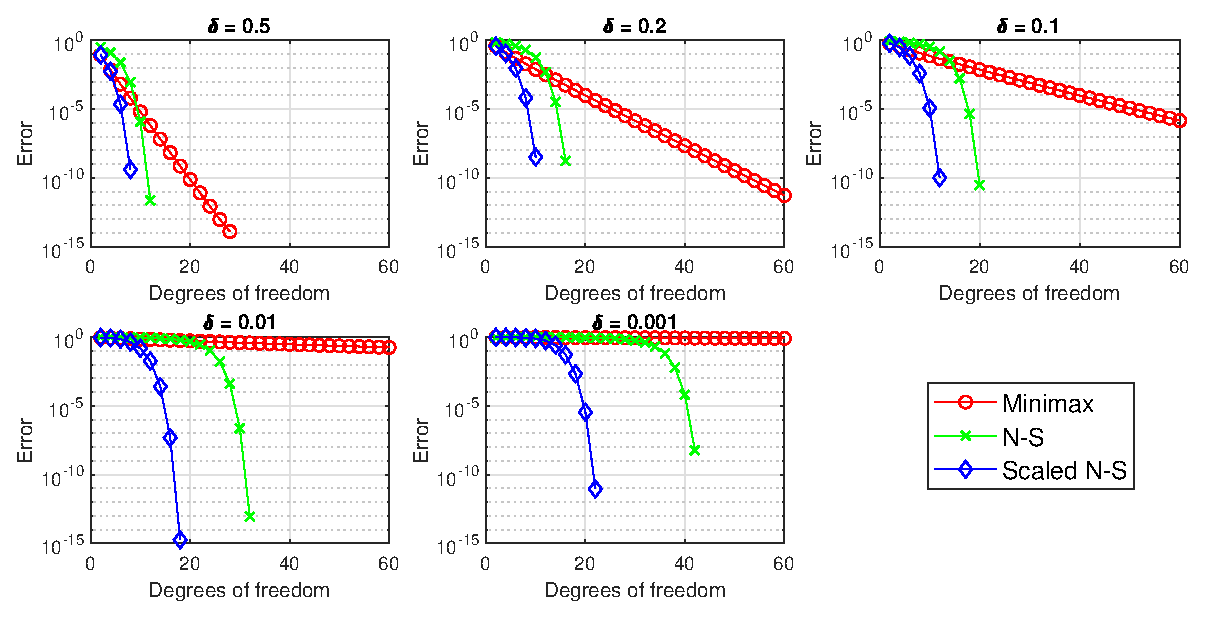
\includegraphics[width=\textwidth,height=\textheight,keepaspectratio]{figures/chapter_3/COMPSIGNvsBEST_DOF_MANY.eps}
   \caption{Error of the unscaled/scaled Newton-Schulz iterates and best approximants to $\sgn(x)$ on $X(\delta)$, with respect to the degrees of freedom, for different values of $\delta$.}
   \label{fig:compsignvsbestDOFmany}
\end{figure}

Comparisons in the error of all the approximations for different values of $\delta$ are shown in Figure \ref{fig:compsignvsbestDOFmany}. For increasingly small values of $\delta$, we observe that the number of iterations required by the unscaled Newton-Schulz iteration in the initial phase of convergence grows faster than that required by the scaled Newton-Schulz iteration. 

%\subsection{Approximating the number of iterations required in the initial convergence phase}

%In this subsection, we compute the approximate number of iterations required by both iterations to obtain an error of $\ep \approx 10^{-1}$, before embarking in some more rigourous analysis shortly. A simple Taylor expansion shows that 
%\[H(x) \sim \dfrac{3\sqrt{3}}{2}x + O(x^2)\] 
%as $x \to 0$, hence we have the approximate error
%\[\ep_k \sim \dfrac{1-C^k \delta}{1+C^k \delta}\]
%as $\delta \to 0$, where $C=3\sqrt3/2$. This is in contrast to the unscaled Newton-Schulz iterates $\tilde{f}_k(x)=g(\tilde{f}_{k-1}(x))$, where $g$ is as in \eqref{scalarNSsign}, which have error $\tilde{\ep}_k:=\tilde{f}_k(\delta)$. By the remark after \cite[Theorem 2.2]{chen}, $\tilde{\ep}_k$ is approximately
%\[\tilde{\ep}_k \sim 1-\left(\dfrac{3}{2}\right)^k \delta\]
%as $\delta \to 0$. Using these relations, we can confirm our first observation about Figure \ref{fig:compsignvsbestDOFmany}, namely that the number of extra iterations required by the unscaled Newton-Schulz approximation grows faster than that required by scaled Newton-Schulz approximation in the initial convergence phase, as $\delta \to 0$. Rearranging for the number of iterations $k$, we find for the scaled Newton-Schulz approximation that 
%\begin{align}
%    k \sim \dfrac{\log\frac{1-\ep}{1+\ep}+\log\frac{1}{\delta}}{\log \frac{3\sqrt{3}}{2}}\label{approx11}
%\end{align}
%iterates are needed for an error of $\ep$, and similarly for the unscaled Newton-Schulz approximation we require
%\begin{align}
%    k \sim \dfrac{\log(1-\ep)+\log\frac{1}{\delta}}{\log \frac{3}{2}}\label{approx22}
%\end{align}
%iterations for an error of $\ep$ in the initial convergence phase. We illustrate this remark in Figure \ref{fig:approxnumberofiterates}, which plots $\delta$ against the approximate number of iterations required by the scaled \eqref{approx11} and unscaled \eqref{approx22} Newton-Schulz iterates to obtain an error of $\ep=0.1$, which is roughly where the convergence seems to start becoming quadratic. Our figure is surprisingly accurate, after cross-checking the number of iterations for $\delta=10^{-p}$, where $p=1,2,3$, with Figure \ref{fig:compsignvsbestDOFmany} (note that DOFs = 2$*$iterations).

%\begin{figure}[t!]
%\centering
%   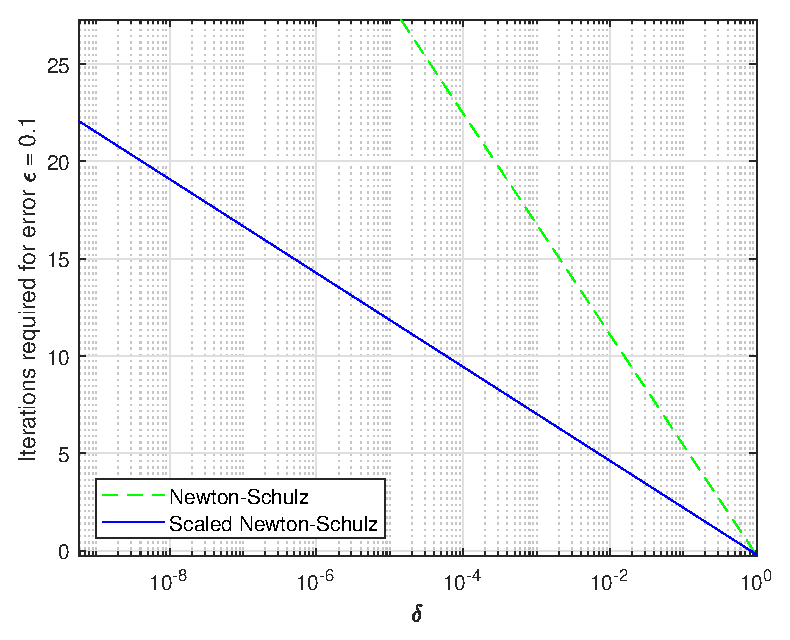
\includegraphics[width=0.7\textwidth,height=0.7\textheight,keepaspectratio]{asymptotic_iteratenumberDOF.eps}
%Newton-Schulz iterations to $\sgn(x)$ to obtain an accuracy of $\ep=0.1$.}
%   \label{fig:approxnumberofiterates}
%\end{figure}

\subsection{Deriving a lower bound for the number of iterations}

To obtain a lower bound for the number of iterations needed to obtain a given accuracy $\ep>0$ for arbitrary $\delta$, it thus seems reasonable to split the convergence analysis into the two phases mentioned in Section \ref{improvednewtonsection}: the initial convergence phase where we reduce the error to a suitably small value, and the asymptotic phase thereafter. We do this by taking inspiration from the analysis conducted by Gawlik and Nakatsukasa (see \cite{Yuji}, or Appendix \ref{compratappendix}).

\bigskip{}

Let $\ep>0$ be the required accuracy. In this subsection, we appropriately select a constant $\delta^* \in (1/e,1)$ and split the convergence into the the following three steps:
\begin{enumerate}
    \item[(1)] find $k_1$ such that $\delta_{k_1} \geq 1/e;$
    \item[(2)] find $k_2$ such that $\delta_{k_1+k_2} \geq \delta^*$;
    \item[(3)] find $k_3$ such that $\ep_{k_1+k_2+k_3} \leq \ep$.
\end{enumerate}

\textbf{Step 1.} Let $k_1$ be the smallest $k$ such that $\delta_k \geq 1/e$. By substituting $x=\delta$ in \eqref{deltak}, we obtain the recursion $\delta_{k+1}=H(\delta_k)$, where
\begin{align}
H(x)=\dfrac{3\sqrt{3}}{2}x\left(\dfrac{1+x}{(1+x+x^2)^{3/2}}\right). \label{hfunction}
\end{align}
A lower bound on $k_1$ is then readily obtained using the following observation.

\begin{lemma}\label{bigdeltalemma}
Let $\delta=\delta_0\in(0,1)$, and define $\delta_{k+1}=H(\delta_k)$ using \eqref{hfunction}. Then
\[\delta_k > \Delta^k \delta\]
for all $k\leq k_1$, where
\[\Delta = \dfrac{H(1/e)}{1/e}\approx 1.928.\]
\end{lemma}

\begin{proof}
Since $H(x)/x$ is strictly decreasing for $x>0$, and $\{\delta_k\}_{k\geq 0}$ is an increasing sequence, it follows that the ratio $\delta_{k+1}/\delta_k$ is also strictly decreasing. In particular, for all $k < k_1$, we have
\begin{align*}
    \dfrac{\delta_{k+1}}{\delta_k}> \dfrac{H(1/e)}{1/e}=\Delta.
\end{align*}
Inductively, it follows that
\[\delta_{k}  >\Delta^{k}\delta_0 = \Delta^{k}\delta\]
for all $k \leq k_1$, as required.
\end{proof}
Choosing $k=k_1$ in Lemma \ref{bigdeltalemma}, we find that $\delta_{k_1}\geq 1/e$ whenever $\Delta^{k_1}\delta\geq 1/e$. As a result, we obtain the lower bound
\[k_1 \geq \dfrac{\log \frac{1}{\delta}-1}{\log\Delta}.\]

%\begin{lemma}\label{taylolemma}
%Given $\delta\in (0,1)$ and $p \in \Pee_3$ defined by \eqref{xis}, we have
%\begin{align}
%    p(x) > \dfrac{3-\delta^2/\xi^2}{2\xi}x,\label{geom}
%\end{align}
%for all $x \in (0,\delta)$.
%\end{lemma}

%\begin{proof}
%This follows trivially, since by definition
%\[p(x)-\dfrac{3-\delta^2/\xi^2}{2\xi}x  = \dfrac{x}{2\xi^3}(\delta^2-x^2) > 0\]
%for all $x \in(0,\delta)$. Geometrically, we interpret the right-hand side of \eqref{geom} as the line through the %origin and $(\delta,p(\delta))$, which lies strictly below $p$ on $(0,\delta)$.
%\end{proof}

%Choosing $\delta=\delta_{k_1}$ and $x=\delta_k$ in Lemma \ref{taylolemma}, where $k_1$ is such that %$\delta_{k_1}\geq 1/e$ and $k < k_1$, we see that
%\[\delta_{k+1} > \dfrac{3-\delta^2_k/\xi_k^2}{2\xi_k} \delta_k\]
%for all $k < k_1$. By definition, this is simply
%\[H(x) > \dfrac{3\sqrt{3}}{2}\left(\dfrac{1+\delta_k}{(1+\delta_k+\delta_k^2)^{3/2}}\right)x.\]
%We have $\delta_{k_1} \gtrsim 1/e$ when
%\[\left(\dfrac{3\sqrt{3}}{2}\right)^{k_1}\delta \gtrsim \dfrac{1}{e},\]
%or equivalently
%\[k_1 \gtrsim \dfrac{\log \frac{1}{\delta}-1}{\log \frac{3\sqrt{3}}{2}}.\]

\textbf{Step 2.} This step no longer depends on $\ep$ or $\delta$, so $k_2$ is a constant. We select $\delta^*$ such that the following lemma holds, as this will help us in step 3. Firstly, define 
\[G(x)=\frac{2\sqrt{x}}{1+x}.\] 

\begin{lemma}\label{hh}
There is $\delta^*\in(0,1)$ such that for every $\delta \in [\delta^*,1]$, there holds
\[\dfrac{1-G(\delta)}{1+G(\delta)}\leq \left(\dfrac{1-\delta}{1+\delta}\right)^2.\]
\end{lemma}

\begin{proof}
As in \cite[Lemma 4.1]{Yuji}. It is shown in \cite[Theorem 3.2]{Gawlik} that the sequence defined by $\alpha_{k+1}=G(\alpha_k)$, where $\alpha_0 \in (0,1)$, is increasing to 1 as $k\to\infty$, and
\[\dfrac{1-G(\alpha_k)}{1+G(\alpha_k)}=\dfrac{1-\alpha_{k+1}}{1+\alpha_{k+1}}=\dfrac{1}{4}\left(\dfrac{1-\alpha_k}{1+\alpha_k}\right)^2+o\left(\left(\dfrac{1-\alpha_k}{1+\alpha_k}\right)^2\right).\]
It follows that
\[\dfrac{1-G(\alpha)}{1+G(\alpha)}\bigg/ \left(\dfrac{1-\alpha}{1+\alpha}\right)^2 \to \dfrac{1}{4}\]
as $\alpha \to 1^-$. Hence $\frac{1-G(\alpha)}{1+G(\alpha)}\big/ \left(\frac{1-\alpha}{1+\alpha}\right)^2$ is bounded by 1 for $\alpha$ sufficiently close to 1.
\end{proof}

\textbf{Step 3.} Let $k_3$ be such that $\ep_{k_1+k_2+k_3} \leq \ep$. To find a lower bound on $k_3$, we will use one final technical lemma.

\begin{lemma}\label{finallemma}
For every $x\in[0,1]$, we have
\[H(x)\leq G(x).\]
\end{lemma}

\begin{proof}
Re-arranging the desired inequality, it suffices to show that
\[J(x):=\dfrac{x(1+x)^4}{(1+x+x^2)^3} \leq \dfrac{16}{27}\]
for all $x \in [0,1]$. Differentiating $J$, we find that
\[J'(x) = \dfrac{(1-x)(x^2+4x+1)(1+x)^3}{(1+x+x^2)^4}\geq 0\]
on $[0,1]$, with equality only when $x=1$. Hence $J$ is bounded by $J(1)=16/27$.
\end{proof}

It follows by Lemma \ref{finallemma} that
\[\dfrac{1-H(\delta_{k})}{1+H(\delta_{k})} \leq \dfrac{1-G(\delta_{k})}{1+G(\delta_{k})},\]
since $x\mapsto \frac{1-x}{1+x}$ is decreasing. By our choice of $\delta^*$, we apply Lemma \ref{hh} to obtain
\[\dfrac{1-\delta_{k+1}}{1+\delta_{k+1}}=\dfrac{1-H(\delta_{k})}{1+H(\delta_{k})} \leq \dfrac{1-G(\delta_{k})}{1+G(\delta_{k})}\leq \left(\dfrac{1-\delta_{k}}{1+\delta_{k}}\right)^2,\]
for $k\geq k_1+k_2$. Inductively, we obtain
\[\dfrac{1-\delta_{k_1+k_2+k}}{1+\delta_{k_1+k_2+k}} \leq \left(\dfrac{1-\delta^*}{1+\delta^*}\right)^{2^k},\]
so we have $\ep_{k_1+k_2+k_3} \leq \ep$ if
\[\left(\dfrac{1-\delta^*}{1+\delta^*}\right)^{2^{k_3}} \leq \ep.\]
Taking logarithms twice, we find
\[k_3 \geq \dfrac{\log\log\frac{1}{\ep}-\log\log\frac{1+\delta^*}{1-\delta^*}}{\log 2}.\]
Combining the all steps, we have that $\ep_k \leq \ep$ when 
\begin{align}
    k \geq  \dfrac{\log \frac{1}{\delta}}{\log \Delta} + \tilde{k}_2 +\dfrac{\log\log\frac{1}{\ep}}{\log 2}, \label{NUMBERITERS}
\end{align}
where $\tilde{k}_2$ is a constant such that
\[\tilde{k}_2 = k_2 - \dfrac{1}{\log \Delta}-\dfrac{\log\log\frac{1+\delta^*}{1-\delta^*}}{\log 2}.\]

%To illustrate the analysis above, we pick a value of $k$ and compute the value of $\delta \in (0,1)$, and thus $\ep_k=\frac{1-\delta_k}{1+\delta_k}$ also, such that the scaled Newton-Schulz iteration $C_k^{-1}f_k$ has approximate error
%\[\norm{C_k^{-1}f_k -\sgn}_{\infty, X(\delta)} \lesssim \ep_k.\]
%Figure \ref{?} demonstrates this for different values of $k$.

%\subsection{Asymptotic behaviour}

%The simplest observation we can make about the scaled Newton-Schulz iterates is what happens as $k \to \infty$. Since $\{\delta_k\}_{k\geq 1}$ is bounded above by $1$, and strictly increasing by Lemma \ref{tekky}, we have $\delta_k \to 1$ as $k\to\infty$. Hence $g_k \to g_$, where
%\[g(x) = \dfrac{x}{2}\left(3-x^2\right),\]
%since $\xi_k \to 1$ also; note that $g$ is precisely the Newton-Schulz iteration function for approximating $\sgn(x)$. Indeed, this shows that convergence is quadratic because $\ep_k \to 0$ quadratically if $\delta_k \to 1$ quadratically, and it follows by similar reasoning to \cite[Theorem 4.2]{chen} we can show that
%\[\lim_{x\to 1}\dfrac{|H(x)-1|}{|x-1|^2} = \lim_{x\to 1} \frac{\left|\frac{3\sqrt{3}}{2}x\left(\frac{1+x}{(1+x+x^{2})^{3/2}}\right)-1\right|}{\left|x-1\right|^{2}}= \dfrac{3}{8}.\]

\subsection{Convergence with respect to degrees of freedom}

In Figure \ref{fig:compsignvsbestDOFmany}, we saw how the scaled Newton-Schulz approximation outperformed the minimax with respect to degrees of freedom. While \eqref{eremboi} shows that the minimax converges exponentially with respect to degrees of freedom, we can use \eqref{NUMBERITERS} to prove that, for any fixed value of $\delta$, the convergence of the scaled Newton-Schulz approximation is \textit{doubly exponential} with respect to degrees of freedom. 

\begin{thm}
Let $\delta \in (0,1)$, and $f_k \in \Pee_{(k,3)}^{\text{comp}}$ be the scaled Newton-Schulz iteration defined by \eqref{deltak}. Then there exist $C_1,C_2>0$ such that
\[\norm{f_k-C_k\emph{\sgn}}_{\infty,X(\delta)} = O(\exp(-C_1 \exp(C_2 d))),\]
where $d=2k$ denotes the number of degrees of freedom of $f_k$.
\end{thm}

\begin{proof}
Equivalently we can show that $\ep_k$, the maximum uniform error of $C_k^{-1}f_k$ to $\sgn$ on $X(\delta)$, is $O(\exp(-C_1 \exp(C_2 d)))$. Increasing $\tilde{k}_2$ until the right-hand side of \eqref{NUMBERITERS} is an integer, and recalling that $f_k$ has degree $3^k$, we find that the degree $n$ of $f_k$ achieving accuracy $\ep_k \leq \ep$, where $\ep >0$, satisfies
\[\dfrac{\log n}{\log 3}=\dfrac{\log \frac{1}{\delta}}{\log \Delta} + \tilde{k}_2 +\dfrac{\log\log \frac{1}{\ep}}{\log 2}.\]
We rearrange this to obtain a bound on $\ep$ as follows:
\begin{align*}
    \log\log\frac{1}{\ep} &= \log 2 \left(\dfrac{\log n}{\log 3}-\dfrac{\log\frac{1}{\delta}}{\log \Delta}-\tilde{k}_2\right)\\
    &=C\log n + D,
\end{align*}
where $C=\log_3 2$ and $D=\log 2\left(\frac{\log\delta}{\log\Delta} - \tilde{k}_2\right)$. Then
\[\log \dfrac{1}{\ep}=\exp(C\log n+D) = \tilde{D} n^C,\]
where $\tilde{D}=e^D$. Finally, we obtain
\begin{align*}
    \ep &= \exp(-\tilde{D}n^C)\\
    &=\exp(-\tilde{D}\exp(C\log n)) \\
    &= \exp(-\tilde{D}\exp(\tilde{C}d)),
\end{align*}
where $\tilde{C}=\frac{1}{2}C\log 3$, since $d=2k=2\log n /\log 3$. Hence the convergence of the scaled Newton-Schulz iteration is doubly exponential with respect to $d$.
\end{proof}
